\subsection{Herramientas}
\label{herramientas-de-visualizacion}

Las herramientas de software de visualización de datos son aquellas que ocupan
de mostrar datos de distintas fuentes en forma de gráficos, de forma que los
usuarios puedan descubrir patrones y entender la información de forma sencilla.

Existen varias herramientas informáticas para visualizar datos. En esta sección
describiremos brevemente a las herramientas \gls{term:kibana} y
\gls{term:grafana}.

\gls{term:kibana} es una plataforma de análisis y visualización de código
abierto diseñada para trabajar con \gls{term:elasticsearch}. Se lo puede usar
para buscar, observar e interactuar con datos almacenados en índices de
\gls{term:elasticsearch}.

Con \gls{term:kibana} es posible realizar análisis de datos complejos y
visualizar datos en una variedad de gráficos, tablas y mapas.
\autoref{fig:kibana}


\begin{figure}
  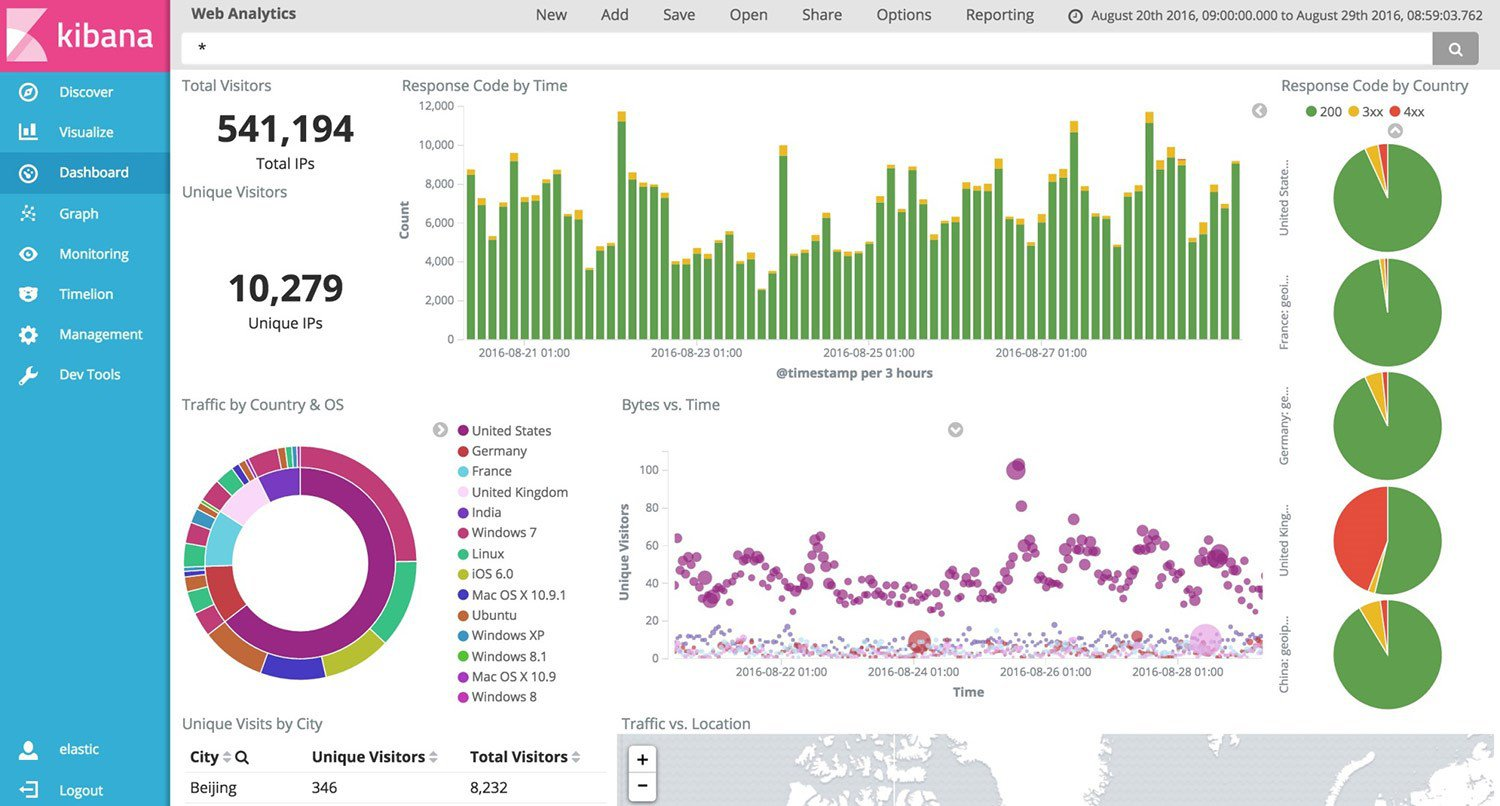
\includegraphics[width=\linewidth]{src/images/05-capitulo-5/kibana.jpg}
  \caption{Tablero de \gls{term:kibana}}
  \label{fig:kibana}
\end{figure}

\gls{term:kibana} cuenta con una interfaz basada en el navegador, que permite
crear y compartir tableros de control dinámicos que muestran los cambios a
consultas de \gls{term:elasticsearch} en tiempo real.

Como hemos mencionado en la teoría, el contar con formas visuales de
representar información permite a las personas entender grandes volúmenes de
datos de forma más sencilla.

\gls{term:grafana} es un tablero y componedor de gráficos de propósito general
y de código abierto que corre como una aplicación \gls{acro:web}. Es comúnmente
usado para visualizar datos de series de tiempo para infraestructuras en la
\gls{acro:web} y analíticas de aplicación, pero también es usado en sensores
industriales, automatización de viviendas, medición del clima y control de
procesos.\autoref{fig:grafana}

\begin{figure}
  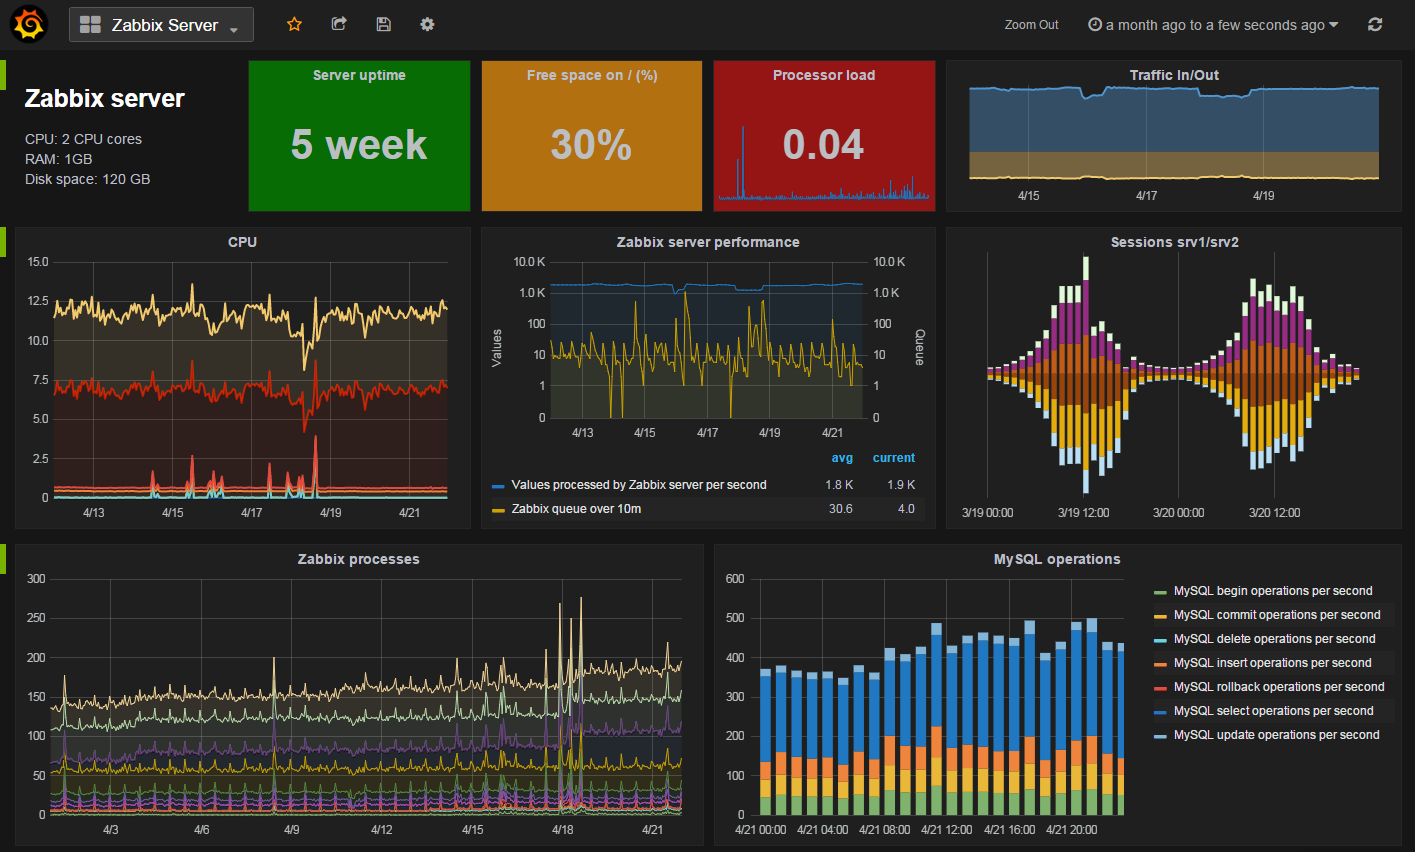
\includegraphics[width=\linewidth]{src/images/05-capitulo-5/grafana.png}
  \caption{Tablero de \gls{term:grafana}}
  \label{fig:grafana}
\end{figure}

\gls{term:grafana} permite una sencilla extensibilidad y variedad de paneles,
con ricas opciones de visualización, y tiene soporte para las fuentes de datos
de series de tiempo más populares, incluyendo \gls{term:influx} y
\gls{term:elasticsearch}.

Luego de analizar estas opciones, nos pareció que la herramienta de
visualización más completa entre ambas era \gls{term:grafana}.

Pero \gls{term:kibana} es un front-end de elasticsearch y está preparado
especialmente para realizar consultas sobre esta base de datos de forma simple.
Con \gls{term:kibana} es posible hacer consultas directas sobre los registros
de logs tal cual fueron recuperados e indexados.

Es por esto que decidimos usar ambas herramientas: \gls{term:kibana} para
consultar las base de datos de \gls{term:elasticsearch}, y hacer consultas
acerca de los logs, y \gls{term:grafana} para comunicarse con nuestra instancia
de \gls{term:influx} y visualizar datos generados en tiempo real.

Creemos importante destacar que estas herramientas están en constante
crecimiento, por lo que no descartamos que en un futuro \gls{term:grafana}
incorpore funcionalidades que se encuentren presentes en \gls{term:kibana}, y
viceversa.
